% B8 · Cold drink — the salted ice bath: model, simulation, handover
% Compile:  xelatex B8-salted-ice-bath.tex   (twice, for references)
% All fonts are loaded from fonts/ beside this file -- nothing needs installing.
% Overleaf: upload the whole folder and set the compiler to XeLaTeX.
\documentclass[11pt,a4paper]{article}

\usepackage{amsmath,amssymb}
\usepackage{fontspec}
\usepackage[math-style=ISO,bold-style=ISO]{unicode-math}
\setmainfont{Inter}[Path=fonts/, Extension=.otf, Scale=0.90,
  UprightFont=*-Regular, ItalicFont=*-Italic, BoldFont=*-SemiBold,
  BoldItalicFont=*-SemiBoldItalic]
\setsansfont{SpaceGrotesk}[Path=fonts/, Extension=.ttf, UprightFont=*-Regular,
  BoldFont=*-Bold, FontFace={m}{n}{*-Medium}]
\setmonofont{JetBrainsMono}[Path=fonts/, Extension=.ttf, UprightFont=*-Regular,
  BoldFont=*-Bold, Scale=0.84, RawFeature={-calt;-liga}]
\setmathfont{latinmodern-math.otf}

\usepackage[a4paper,top=24mm,bottom=26mm,left=24mm,right=24mm]{geometry}
\usepackage{xcolor}
\definecolor{teal}{HTML}{0F766E}
\definecolor{orange}{HTML}{C2410C}
\definecolor{ink}{HTML}{1F2937}
\definecolor{grey}{HTML}{6B7280}
\definecolor{light}{HTML}{F3F4F6}
\definecolor{teall}{HTML}{E6F4F2}
\definecolor{orangel}{HTML}{FDEEE6}
\color{ink}

\usepackage{graphicx,booktabs,tabularx,array,enumitem,caption,listings}
\usepackage[hidelinks]{hyperref}
\usepackage{titlesec}
\titleformat{\section}{\sffamily\Large\bfseries}{\color{teal}\thesection}{0.7em}{}
\titleformat{\subsection}{\sffamily\large\fontseries{m}\selectfont}{\color{teal}\thesubsection}{0.6em}{}
\titleformat{\paragraph}[runin]{\sffamily\bfseries}{}{0pt}{}[.]
\titlespacing*{\section}{0pt}{1.6ex plus .5ex}{0.9ex}
\titlespacing*{\subsection}{0pt}{1.2ex plus .4ex}{0.6ex}
\setlength{\parindent}{0pt}
\setlength{\parskip}{0.55em}
\linespread{1.08}
\captionsetup{font={small}, labelfont={sf,bf,color=teal}, labelsep=period, skip=4pt}
\setlist{itemsep=2pt, topsep=2pt, leftmargin=1.3em}
\renewcommand{\arraystretch}{1.16}

\lstset{basicstyle=\ttfamily\footnotesize, columns=fullflexible, keepspaces=true,
  numbers=left, numberstyle=\ttfamily\scriptsize\color{grey}, numbersep=6pt,
  commentstyle=\color{teal}, stringstyle=\color{orange}, keywordstyle=\bfseries,
  language=Python, frame=l, framerule=1.2pt, rulecolor=\color{teal},
  backgroundcolor=\color{light}, xleftmargin=2.2em, aboveskip=6pt, belowskip=4pt}

\newcommand{\dC}{\,^{\circ}\mathrm{C}}
\newcommand{\code}[1]{\texttt{#1}}
\newfontfamily\symfont{DejaVuSans}[Path=fonts/, Extension=.ttf, Scale=0.9]
\newcommand{\secsrc}{{\symfont ◐}}
\newcommand{\FLOOR}{\textcolor{teal}{\textsf{\bfseries FLOOR}}}
\newcommand{\RATE}{\textcolor{orange}{\textsf{\bfseries RATE}}}

\begin{document}

% ---------------------------------------------------------------- title
{\sffamily
{\color{teal}\small\bfseries SYPT 2027 · PROBLEM B8 · COLD DRINK}\\[3pt]
{\Huge\bfseries The Salted Ice Bath}\\[4pt]
{\large A model of the bath and the drink, with a working simulation}\\[2pt]
{\color{grey}Handover report — October 2026 · built from the Drive file \code{sypt code}}\par
}
\vspace{4pt}
\noindent{\color{teal}\rule{\linewidth}{1.2pt}}\par

A drink is cooled in an ice\,:\,water\,:\,salt bath. This report closes the calculation that the
script \code{sypt code} began, turns it into a time-dependent simulation of the drink and the
bath together (\code{b8\_sim.py}), and records what the simulation says about the rig built on
20 October. Two parts of the problem keep the colour code used in the reporter deck:
\FLOOR\ (equilibrium thermodynamics — how cold) and \RATE\ (heat transfer — how fast). No new
measurements were taken; every number below is printed by running \code{python3 b8\_sim.py},
and §1 says which parts are solid. §8 contains a result that changes the rig: \textbf{the
charge specified in the rig note does not reach the eutectic}, so it has no thermostat.
§\ref{sec:spread} describes the time-dependent model behind the interactive simulator
(\code{b8\_model.py}), in which ice melts and salt dissolves at finite rates and the drink's heat
spreads through the bath no faster than the brine carries it: \textbf{that spreading alone
lengthens the time to 5\,°C from 212 to 246\,s.} It also counts, path by path, the heat that
leaks in through the styrofoam box, which is not a perfect insulator, and gives a test to
measure that leak.

% ---------------------------------------------------------------- 1
\section{Status of the work}

\textbf{Solid.} The enthalpy formulation (§4) and the equilibrium solve it implies; the
reproduction of every bath number in the earlier B8 notes once their starting temperatures are
matched (Table~\ref{tab:repro}); the result that the bath temperature cannot be found from
composition alone, which is why the original \code{temp()} could not be finished; the
$1/\text{size}$ scaling of bath drift; the condition for reaching the eutectic adiabatically
(§6.3); and the numerical integrator, which matches both closed-form cooling laws to five
figures and conserves energy to $10^{-6}$ relative.

\textbf{Computed but not measured.} The adiabatic temperature of any charge; the buffer map
(Fig.~\ref{fig:map}); the drink cooling curves for the measured Can~2; the blank-run warming
rate and the error made by inverting it with $L_f$ instead of $L_{\text{eff}}$.

\textbf{Uncertain.} The overall heat-transfer coefficient $U_0 = 160$\,W\,m$^{-2}$K$^{-1}$,
taken from the SINTEF time constant rather than measured on this rig — every \RATE\ number
scales with it. The heat capacities and dissolution enthalpy are textbook placeholders; §11.4
shows the \FLOOR\ results move by at most 0.3\,K when they are varied over a plausible range.
The convection factor that sets how fast the drink's heat spreads through the bath
(§\ref{sec:spread}) is an estimate; over 5–100 it moves the time to 5\,°C from 286.5 to 222\,s.
So is the box's leak, worked out as 0.34\,W\,K$^{-1}$ (§\ref{sec:box}); it barely moves the drink,
but it sets how fast the bath warms, and the box test measures it.

\textbf{Not attempted.} Stratification of the bath (§\ref{sec:spread} resolves it around the
can, not in height); the metastable eutectic and hydrohalite nucleation; freezing or
supercooling of the drink in \code{b8\_sim.py} (\code{b8\_model.py} has both); flow inside the
drink (the COMSOL model covers that); and any dissolution law that could explain the bench stall
at $-7.5\dC$ (§9).

% ---------------------------------------------------------------- 2
\section{Starting point: what \code{sypt code} did}

The script defines the right ingredients — 1\,kg ice, 2\,kg water, 0.5\,kg salt, $L_f =
333.55$\,kJ\,kg$^{-1}$, $K_f = 1.86$\,K\,kg\,mol$^{-1}$, $i = 2$, and a linear solubility fit
from the Sigma-Aldrich table — and stops. Read bluntly:

\begin{center}\small
\begin{tabularx}{\linewidth}{@{}>{\raggedright}p{0.25\linewidth}X@{}}
\toprule
\textbf{Line} & \textbf{Problem, and what it costs} \\ \midrule
\code{bathT = 25.0 \#\# K} & It is 25\,°C. 25\,K is $-248\dC$. Every temperature in the model is Celsius; the label should say so. \\
\code{solubility()} & Compares \code{paramsaltMass} in kg with a fit in \emph{grams per 100\,g of water}. 0.5 is always less than 35.2, so the cap can never bind, for any input. Correct form: $s_{\max} = 10^{-2}\,(0.0338\,T + 35.24)\,m_w$ kg. The fit is also the \emph{halite} branch, valid above $+0.1\dC$; below that the solid in equilibrium is hydrohalite and the solubility falls to 30.2\,g/100\,g at the eutectic, not the 34.5 the fit extrapolates to. \\
\code{temp()} & Computes $\Delta T_f$ and returns nothing, so the function evaluates to \code{None}. \\
molality in \code{temp()} & Divides by the initial 2\,kg of water. The liquid water at equilibrium is 2\,kg \emph{plus whatever ice melted}, and that is the unknown. \\
Blagden, $i = 2$ & Over-predicts the depression by 11\,\% at 5\,wt\,\%, under-predicts by 9\,\% near the eutectic (§6.1), and has no floor: at 30\,wt\,\% it gives $-27.3\dC$ for a brine that cannot exist. \\
\code{1.201 Density ... as a \%} & Density is in g\,mL$^{-1}$, not a percentage. Unused, but \code{waterVol} is used as a mass: fine for water, 20\,\% wrong for brine. \\
\code{import matplotlib}, \code{time} & \code{pyplot} is never imported; \code{main()} times nothing. Harmless. \\
\bottomrule
\end{tabularx}
\end{center}

The one that matters is structural, not a bug. \textbf{The temperature depends on the brine
composition, the composition depends on how much ice has melted, and how much ice melts depends
on the temperature.} Composition alone cannot close that loop; an energy balance can. For the
script's own charge, \code{temp()} would have reported $-15.9\dC$ (20\,wt\,\%, all salt in the
original 2\,kg). The equilibrium is $-13.7\dC$ with 647\,g of ice left if the water starts at
0\,°C, and $-10.5\dC$ with only 51\,g of ice left if it starts at 25\,°C — a bath one cold drink
away from running out of ice. Everything below is the loop closed.

% ---------------------------------------------------------------- 3
\section{Coordinates and variables}

\textbf{State variables} — what the simulation integrates.

\begin{center}\small
\begin{tabularx}{\linewidth}{@{}l l X@{}}
\toprule
$H_b$ & kJ & total enthalpy of the bath (ice + brine + solid salt) \\
$T_d$ & °C & drink temperature, lumped \\
$s$ & kg & dissolved salt — a state variable only in kinetic runs (§9); otherwise fixed by equilibrium \\
\bottomrule
\end{tabularx}
\end{center}

\textbf{Determined by the state} through the equilibrium solve $\mathcal T$ (§4.3).

\begin{center}\small
\begin{tabularx}{\linewidth}{@{}l l X@{}}
\toprule
$T_b$ & °C & bath temperature, one value for the whole bath \\
$m_i$, $m_l$ & kg & ice, and liquid water in the brine; $m_i + m_l = W$ \\
$s$, $S - s$ & kg & dissolved and undissolved salt \\
$w = s/(m_l+s)$ & – & brine mass fraction \\
regime & – & \code{liquid} / \code{liquidus} / \code{eutectic} / \code{solid} \\
\bottomrule
\end{tabularx}
\end{center}

\textbf{Fixed.} Totals $W$ (all water, as ice or liquid) and $S$ (all salt); starting
temperatures of ice, water and salt; drink heat capacity $C_d$; drink area $A$ and
coefficient $U_0$; box conductance $(UA)_{\text{box}}$ and room temperature $T_{\text{env}}$.

\begin{center}\small
\begin{tabular}{@{}l r l l@{}}
\toprule
Constant & Value & Unit & Status \\ \midrule
$L_0$ (ice, 0\,°C) & 333.55 & kJ\,kg$^{-1}$ & as in \code{sypt code} \\
$c_w$, $c_i$, $c_s$ & 4.18, 2.00, 0.864 & kJ\,kg$^{-1}$K$^{-1}$ & $c_i$ assumed (2.05 at 0, 1.94 at $-20\dC$) \\
$c_b(w)$ & $4.18 - 4.4\,w$ & kJ\,kg$^{-1}$K$^{-1}$ & assumed, room-temperature values \\
$\Delta h_s$ & $+66.4$ & kJ\,kg$^{-1}$ & 3.88 kJ\,mol$^{-1}$, infinite dilution, 25\,°C \\
$T_E$, $w_E$ & $-21.2$, 0.2318 & °C, – & Bodnar fit end point \\
$T_P$, $w_P$ & $+0.1$, 0.26285 & °C, – & Swenne (1983) peritectic \\
$C_d$ & 1.332 & kJ\,K$^{-1}$ & 330\,g drink at $c = 4.0$ + 13\,g Al; to be weighed \\
$A$ & 0.03102 & m$^2$ & Can~2, measured 20 Oct \\
$U_0$ & 160 & W\,m$^{-2}$K$^{-1}$ & from SINTEF $\tau \approx 265$\,s; to be measured \\
$(UA)_{\text{box}}$, $T_{\text{env}}$ & 0.46, 28 & W\,K$^{-1}$, °C & rig note, 30\,mm EPS \\
\bottomrule
\end{tabular}
\end{center}

% ---------------------------------------------------------------- 4
\section{The model}

\subsection{One idea}
The bath is described by its enthalpy, not its temperature. Heat that crosses the bath boundary
changes $H_b$; everything else — temperature, ice remaining, brine composition, salt left on
the floor — is read off $H_b$ by an equilibrium solve. Five behaviours that are usually bolted on
as separate rules then come out of one function: the adiabatic mixing temperature, drift along
the liquidus as ice melts, the eutectic thermostat, ice exhaustion, and the temperature
dependence of the latent heat.

\subsection{Enthalpy and phase closures}
Reference state: liquid water and solid NaCl at 0\,°C have zero enthalpy.
\begin{equation}
H = \underbrace{(m_l+s)\,c_b(w)\,T}_{\text{brine, sensible}}
  + \underbrace{s\,\Delta h_s}_{\text{dissolution}}
  + \underbrace{m_i\,(c_i T - L_0)}_{\text{ice}}
  + \underbrace{(S-s)\,c_s T}_{\text{undissolved salt}}
\label{eq:H}
\end{equation}
The liquidus is Bodnar's empirical fit, with $\theta = -T$ the final ice-melting temperature,
\begin{equation}
w_L(T) = 0.0178\,\theta - 4.42\times10^{-4}\,\theta^2 + 5.572\times10^{-6}\,\theta^3,
\qquad 0 \le \theta \le 21.2,
\label{eq:bodnar}
\end{equation}
explicit in $T$, which is what makes the solve fast. Solubility has two branches: the
script's own fit above $T_P$, and a straight line from $(T_P, w_P)$ to $(T_E, w_E)$ below it.
Eutectic brine carries $r_E = w_E/(1-w_E) = 0.3018$\,kg of salt per kg of water.

\subsection{The equilibrium solve $T_b = \mathcal T(H_b;\,W, S)$}
\begin{center}\small
\begin{tabularx}{\linewidth}{@{}l X l@{}}
\toprule
Regime & Phase amounts & $T_b$ \\ \midrule
\code{liquid} & $m_i = 0$,\; $s = \min\!\big(S,\; W\,r_{\text{sat}}(T)\big)$ & from \eqref{eq:H} \\
\code{liquidus} & $w = w_L(T)$,\; $s = S$,\; $m_l = S\,(1-w_L)/w_L$,\; $m_i = W - m_l$ & from \eqref{eq:H} \\
\code{eutectic} & $w = w_E$,\; $0 \le m_l \le \min(W, S/r_E)$,\; $s = r_E\,m_l$ & $T_E$, fixed \\
\code{solid} & no liquid & below $T_E$ \\
\bottomrule
\end{tabularx}
\end{center}
On the \code{liquidus} branch all available salt is dissolved, because the liquidus lies
below saturation everywhere above $T_E$; undissolved salt and ice can only coexist at $T_E$.
$H(T)$ is continuous and strictly increasing across the \code{liquid}/\code{liquidus} boundary,
so the root is unique and bracketed on $(T_E, 200\dC)$. On the plateau $H$ is linear in $m_l$,
so the solve there is a single division. \eqref{eq:H} is evaluated at both ends of the plateau
with the same $w_E$ — computed from \eqref{eq:bodnar}, not typed — or the branch and plateau
fail to meet by $10^{-3}$\,kJ and the bracket breaks.

\subsection{Equations of motion}
\begin{align}
C_d\,\dot T_d &= -\,U A\,(T_d - T_b)
  \label{eq:drink}\\
\dot H_b &= \underbrace{U A\,(T_d - T_b)}_{\text{from the drink}}
  + \underbrace{(UA)_{\text{box}}\,(T_{\text{env}} - T_b)}_{\text{leak}}
  + \underbrace{P_{\text{stir}}}_{\text{stirrer}},
\qquad T_b = \mathcal T(H_b)
  \label{eq:bath}
\end{align}
with either $U = U_0$ (Newton) or $U = U_0\,(|T_d-T_b|/\Delta T_0)^{1/4}$, $\Delta T_0 = 25$\,K,
the free-convection law from the equation bank. Salt added mid-run enters as $\Delta S$ and
$\Delta H = \Delta S\,c_s T_{\text{env}}$. The pair is integrated by Heun's method at
$\Delta t = 0.25$\,s.

\subsection{Scales}
\begin{equation}
\tau = \frac{C_d}{UA} = 268\ \text{s},\qquad
t_{\text{target}} = \tau \ln\frac{T_{d0}-T_b}{T_{\text{target}}-T_b},\qquad
\theta(t) = \theta_0\Big(1+\frac{t}{t^*}\Big)^{-4},\;\;
t^* = 4\tau\Big(\frac{\Delta T_0}{\theta_0}\Big)^{1/4}
\label{eq:scales}
\end{equation}
the second for a constant bath under Newton's law, the third its power-law counterpart with
$\theta = T_d - T_b$. Both are used as checks on the integrator, not as the model.

% ---------------------------------------------------------------- 5
\section{Where the model comes from}

\subsection{Why enthalpy, and why it is unique}
With ice present the brine must sit on the liquidus, so $T_b$ and $w$ are one unknown, and
$m_l$ follows from the salt balance $s = w\,(m_l+s)$. The only remaining unknown is fixed by
energy. Fixing $H$ instead of $T$ removes the circularity of §2: given $H$ the state is
determined, and the bath's temperature is a consequence. Gibbs' phase rule says the same thing
from the other side — two components and three phases (ice, brine, salt) leave
$F = C - P + 1 = 0$ degrees of freedom at fixed pressure, so on the eutectic $T$ cannot move
and heat can only change the phase amounts.

\subsection{The latent heat that the bath actually charges}
Holding $S$ fixed on the liquidus, $m_l = S(1-w)/w$ gives $\mathrm d w/\mathrm d m_{\text{melt}} = -w^2/S$, so
\begin{equation}
\frac{\mathrm dT_b}{\mathrm dm_{\text{melt}}} = \frac{w^2}{S\,\lvert w_L'(T_b)\rvert},
\qquad
L_{\text{eff}} \equiv \frac{\mathrm dH}{\mathrm dm_{\text{melt}}}
 = \underbrace{L_0 + (c_b - c_i)\,T_b}_{L(T_b)}
 + \underbrace{C_{\text{bath}}\,\frac{\mathrm dT_b}{\mathrm dm_{\text{melt}}}}_{\text{warming the bath}} .
\label{eq:Leff}
\end{equation}
The first term is the latent heat at the bath temperature, which falls below $L_0$; the second
is the heat spent warming every kilogram of the bath along the liquidus while a kilogram of ice
melts. \eqref{eq:H} contains both automatically; the code evaluates $L_{\text{eff}}$ by
finite difference in $H$, so no separate correction is needed. Both factors in
$\mathrm dT_b/\mathrm dm$ carry $1/S$: double every mass and the drift per kilogram melted
halves. That is the $1/\text{size}$ law of the rig note, now derived.

\subsection{Where the cold comes from}
Integrating \eqref{eq:H} between the unmixed and mixed states, the heat that cools the bath is
paid by two terms only: $L(T)\,m_{\text{melt}}$ and $s\,\Delta h_s$. Their ratio is read off
any equilibrium.

% ---------------------------------------------------------------- 6
\section{Analytical consequences}

\subsection{The original formula against the data}
\FLOOR. Blagden's law, $T = -2K_f\,b$ with $b = 1000\,w/[M(1-w)]$, crosses Bodnar's
liquidus at \textbf{16.5\,wt\,\% / $-12.61\dC$}, the dossier's value to rounding. The ratio of
ideal to measured depression is 1.106, 1.069, 1.019, 0.952, 0.909 at 5, 10, 15, 20,
23\,wt\,\% (Fig.~\ref{fig:liq}). As the first-principles note warned, the location of the
crossing belongs to the linear formula; a fuller ideal-solution calculation crosses near
12\,wt\,\%.

\subsection{Pre-dissolving has a floor near $-13\dC$}
Salt dissolved in water at room temperature spends its $\Delta h_s$ cooling water that the room
then rewarms, and the brine arrives at the ice carrying sensible heat that can only be paid in
meltwater, which dilutes it. For the five pre-dissolved recipes in the 10 Sep notes the model
gives $-12.0$ to $-12.5\dC$ (notes: $-12.1$ to $-12.6$); \textbf{saturating the brine at 25\,°C
moves the floor only to $-12.9$ to $-13.1\dC$}. The 10 Sep conclusion — the eutectic needs
staged addition onto ice — follows, and the staged protocol 20\,+\,6\,+\,6\,+\,6\,g reproduces as
$-12.4$, $-15.8$, $-19.1$, $-21.2\dC$ (notes: $-12.4$, $-15.7$, $-18.9$, $-21.2$).

\subsection{Reaching the eutectic is an energy condition, not a mass condition}
A charge reaches the thermostat only if its starting enthalpy lies below the top of the plateau,
\begin{equation}
H_0 \;\le\; H\big(T_E;\; m_l = \min(W,\,S/r_E)\big),
\label{eq:reach}
\end{equation}
and keeps solid salt only if it lies further below. Free water is expensive: every kilogram
must be cooled to $-21.2\dC$ and salted to $w_E$, and the only payment is melting ice, which
brings more water. For 5.6\,kg of water in total, 1.0\,kg of salt, water at 4\,°C: the ice
fraction must exceed \textbf{0.612} to reach $T_E$ and \textbf{0.691} to keep 150\,g of salt
solid (ice at 0\,°C); 0.555 and 0.627 with ice from a $-18\dC$ freezer (Fig.~\ref{fig:map}).
Checking that the salt saturates the free water — the rig note's test — is necessary and not
sufficient.

\subsection{Drift and the buffer}
On the liquidus, 300\,g of salt at 20\,wt\,\% gives $+17.3$\,K per kg melted (equation bank:
$+17$). Rebuilding the rig note's four baths on their own liquidus and melting 150\,g gives
$+5.91$, $+1.85$, $+0.97$, $+0.49$\,K, its table to two decimals. On the plateau, forming
1\,kg of eutectic brine absorbs \textbf{241\,kJ} and consumes 0.960\,g of solid salt per kJ.
The rig note's 272\,kJ\,kg$^{-1}$ used $L_0$ at 0\,°C; at $-21.2\dC$ the latent heat is lower,
so the buffer is used up \textbf{13\,\% faster} than that note assumed.

\subsection{Rate and floor optimise at different loadings}
\RATE\ and \FLOOR\ part company (Fig.~\ref{fig:cool}b). For 4\,kg ice and 1.6\,kg water, time to
5\,°C falls with salt until the starting bath reaches $T_E$ at salt\,:\,ice $\approx 0.20$
(2.82\,min) and is flat beyond. The drink temperature after 40\,min keeps falling until
$\approx 0.23$, where enough solid salt survives the drink and 40\,min of leak to keep the bath
pinned. Beyond that, more salt buys only hold time.

% ---------------------------------------------------------------- 7
\section{Numerical results}

\begin{figure}[t]
\centering
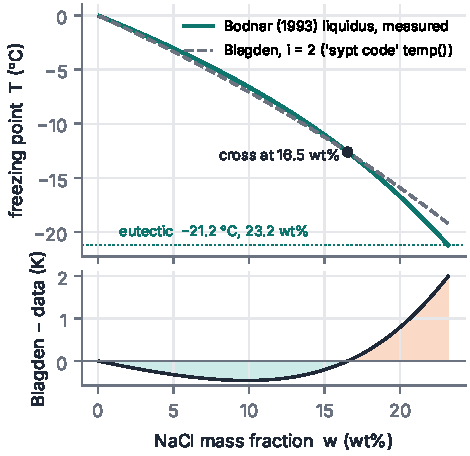
\includegraphics[width=0.56\linewidth]{figs/f1_liquidus.pdf}
\caption{\FLOOR. Freezing point against composition: Bodnar's measured liquidus and Blagden's
law as coded in \code{temp()}. Lower panel: Blagden minus data. The residual is small for the
dilute brines and grows to 2.0\,K at the eutectic, where Blagden also loses the floor.}
\label{fig:liq}
\end{figure}

\begin{table}[t]
\centering\small
\caption{Reproduction of earlier B8 numbers. Each earlier number assumed a starting temperature
it did not state; the column says which one reproduces it.}
\label{tab:repro}
\begin{tabularx}{\linewidth}{@{}>{\raggedright\arraybackslash}X l l l@{}}
\toprule
Case & Notes & This model & Start \\ \midrule
75\,g ice + 25\,g water + 18\,g salt & eutectic, $\sim$2\,g solid & $-21.2\dC$, 2.7\,g solid & 25\,°C water \\
stall at $-7.5\dC$ forces $w$ & 11.1\,wt\,\% & 11.1\,wt\,\% & – \\
150 + 60 + 20 pre-dissolved & $-12.4\dC$ & $-12.42\dC$ & 25\,°C brine \\
staged 20 + 6 + 6 + 6\,g & $-12.4/-15.7/-18.9/-21.2$ & $-12.4/-15.8/-19.1/-21.2$ & 25\,°C \\
1200 ice + 400 water, 20\,g salt & $-2.07\dC$ & $-2.08\dC$ & 25\,°C water \\
\quad … 90\,g / 200\,g & $-8.61$ / $-17.58\dC$ & $-8.67$ / $-17.92\dC$ & 25\,°C water \\
Blagden crossover & 16.4–16.5\,wt\,\% & 16.5\,wt\,\% & – \\
drift, four bath sizes & $+5.91/1.86/0.97/0.49$ K & $+5.91/1.85/0.97/0.49$ K & on liquidus \\
$L_{\text{eff}}/L_f$ & 1.15–1.70 & 1.15 at $-11.2\dC$ & – \\
latent share of the cold & $\sim$92\,\% & 87\,\% (0\,°C) to 90–92\,\% (25\,°C) & see note \\
\bottomrule
\end{tabularx}
\end{table}

Where a number does not reproduce, the starting temperature is the reason. With the water
at 0\,°C instead of 25\,°C the Session-1 sweep runs 0.6–3.3\,K colder at every step, and the
latent share drops to 87\,\%: warm free water must be paid for by melting ice, which raises the
latent share. The earlier 92\,\% therefore belongs to a warm-water charge. The conclusion is
unchanged — the salt supplies about a tenth of the cold and the ice the rest — but the earlier
notes should state their starting temperatures.

\begin{figure}[t]
\centering
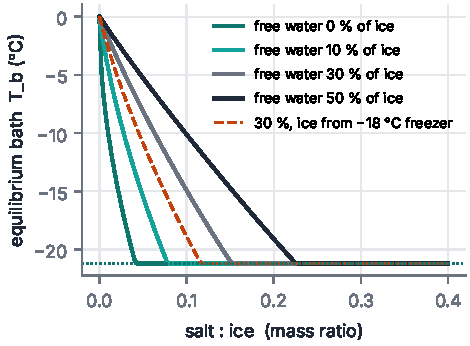
\includegraphics[width=0.49\linewidth]{figs/f2_recipe.pdf}\hfill
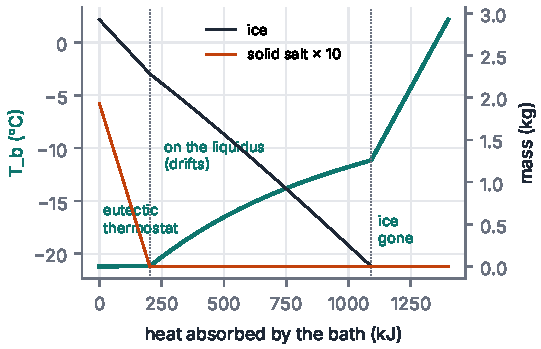
\includegraphics[width=0.49\linewidth]{figs/f3_charge.pdf}
\caption{\FLOOR. \emph{Left:} adiabatic bath temperature against salt\,:\,ice, ice at 0\,°C.
More free water needs more salt to reach the floor; at 30\,\% free water, $-18\dC$ freezer ice cuts the salt needed from 0.15 to 0.12.
\emph{Right:} the buffered charge (§8) as heat is added. Three regimes in order: the plateau,
where solid salt is consumed at fixed $T_E$; the liquidus, where the bath drifts as ice
melts; ice exhausted, where it warms freely.}
\label{fig:recipe}
\end{figure}

\begin{figure}[t]
\centering
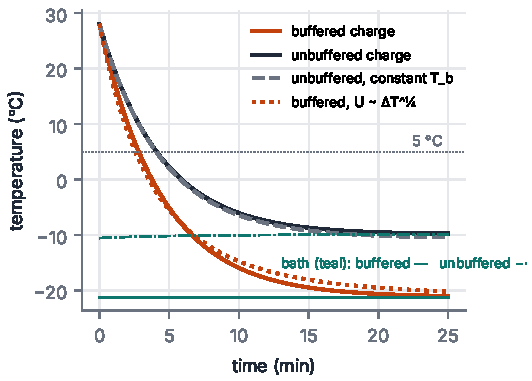
\includegraphics[width=0.49\linewidth]{figs/f4_cooling.pdf}\hfill
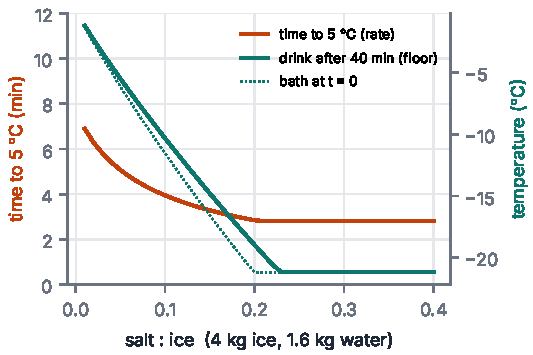
\includegraphics[width=0.49\linewidth]{figs/f5_rate_floor.pdf}
\caption{\RATE. \emph{Left:} Can~2 from 28\,°C in three charges. The buffered bath holds
$-21.2\dC$ throughout; the unbuffered one warms by 0.7\,K, and the constant-$T_b$ model
misses that by 2.2\,s in time to 5\,°C. The dotted curve is the $\Delta T^{1/4}$ law.
\emph{Right:} time to 5\,°C (rate) and drink temperature after 40\,min (floor) against salt;
they saturate at 0.20 and 0.23.}
\label{fig:cool}
\end{figure}

\begin{figure}[t]
\centering
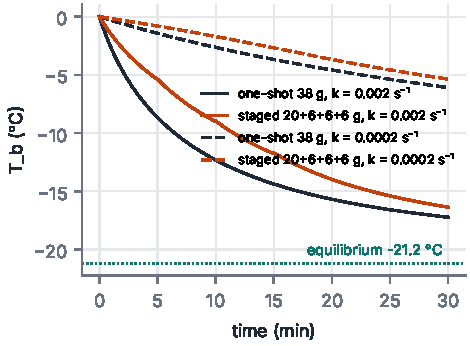
\includegraphics[width=0.49\linewidth]{figs/f6_kinetics.pdf}\hfill
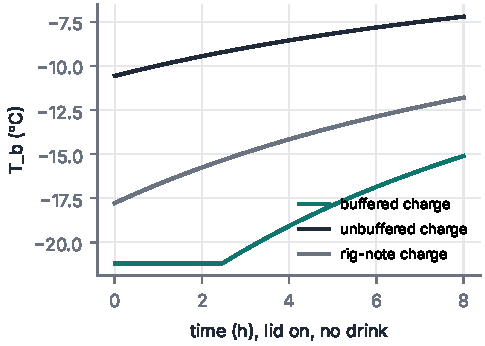
\includegraphics[width=0.49\linewidth]{figs/f7_blank.pdf}
\caption{\emph{Left:} well-mixed kinetic dissolution, 150\,g ice + 60\,g water, same 38\,g of
salt added at once or in four tranches, for two rate constants. One-shot is \emph{faster} in
this model — the opposite of the bench (§9). \emph{Right:} blank runs, lid on, no drink. The
buffered charge holds the plateau for 2.5\,h on the leak alone.}
\label{fig:kin}
\end{figure}

\begin{figure}[t]
\centering
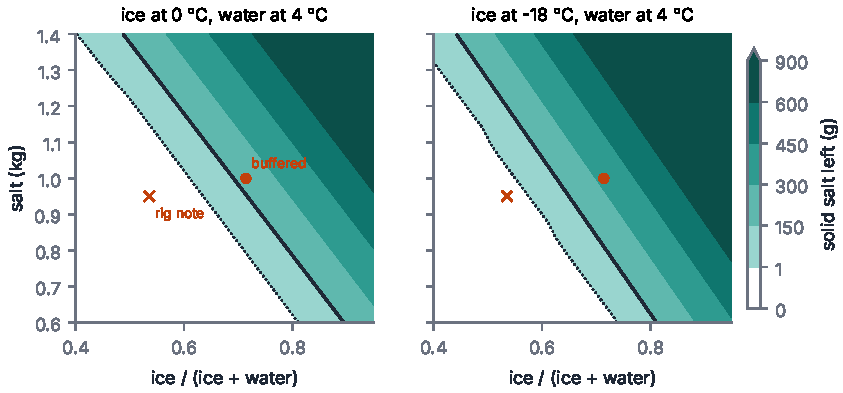
\includegraphics[width=0.92\linewidth]{figs/f8_buffer_map.pdf}
\caption{\FLOOR. Solid salt left at adiabatic equilibrium, 5.6\,kg of water in total, water at
4\,°C, salt at 28\,°C. White: never reaches $T_E$. Dotted: just reaches it. Solid line: 150\,g
of salt stays solid. Cross: the rig-note charge. Dot: the buffered charge of §8.}
\label{fig:map}
\end{figure}

% ---------------------------------------------------------------- 8
\section{Numbers for the rig}

Tank 7.21\,L, Can~2 ($\varnothing$\,66.0\,mm, 116.6\,mm, $A = 310.2$\,cm$^2$), 330\,g of drink,
EPS box at 0.46\,W\,K$^{-1}$, room 28\,°C, drink from 28\,°C. Ice at 0\,°C, water at 4\,°C, salt
at room temperature.

\begin{center}\small
\begin{tabular}{@{}l c c c@{}}
\toprule
& rig note & \textbf{buffered} & unbuffered \\
& 3.0\,:\,2.6\,:\,0.95\,kg & \textbf{4.0\,:\,1.6\,:\,1.00\,kg} & 3.0\,:\,2.6\,:\,0.55\,kg \\ \midrule
starting $T_b$ & $-17.78\dC$ & $\mathbf{-21.20\dC}$ & $-10.57\dC$ \\
regime & liquidus & eutectic & liquidus \\
solid salt at start & 0\,g & 193\,g & 0\,g \\
time to 5\,°C (Newton) & 189\,s & 169\,s & 246\,s \\
\quad $\Delta T^{1/4}$ law & – & 155\,s & – \\
$T_b$ after 25\,min & $-16.50\dC$ & $-21.20\dC$ & $-9.86\dC$ \\
ice melted / salt used in 25\,min & 222\,g / – & 316\,g / 95\,g & 204\,g / – \\
blank-run warming & 1.13\,K\,h$^{-1}$ & 0 for 2.5\,h & 0.62\,K\,h$^{-1}$ \\
\bottomrule
\end{tabular}
\end{center}

\textbf{The rig-note charge has no thermostat.} It saturates its free water, which is what the
rig note checked, but adiabatically it lands at $-17.8\dC$ with every gram of salt dissolved,
and even with $-18\dC$ freezer ice only at $-19.5\dC$. The “$\geq 150$\,g stays solid” line was
a mass balance; the energy balance \eqref{eq:reach} says otherwise. \textbf{Use 4.0\,kg ice +
1.6\,kg water + 1.0\,kg salt}: $-21.2\dC$ with 193\,g solid, an equilibrium volume of about
6.2\,L, plus 0.40\,L for the can, inside the 6.8\,L to the 16.5\,cm line. Add the ice in two lots;
4\,kg of crushed ice heaps above the brim until the first lot melts back. One drink plus 25\,min
of leak uses 95\,g of the 193\,g, so top up the salt between runs and watch for crystals on the
floor.

\textbf{The blank-run inversion needs $L_{\text{eff}}$.} Inverting the warming rate as
$\dot Q = L\,\dot T_b/(\mathrm dT_b/\mathrm dm)$ recovers the true 17.7\,W leak of the unbuffered
charge as 15.5\,W with $L_f$ ($-13\,\%$) and 17.6\,W with $L_{\text{eff}}$ ($-1\,\%$); for the
rig-note charge, 16.9 against 21.1\,W ($-20\,\%$) and 20.8\,W ($-1\,\%$). Fit the slope over the
first ten minutes: $\mathrm dT_b/\mathrm dm$ itself falls as the bath dilutes, so a one-hour
average biases the answer by another 5\,\%. And the buffered bath cannot be used for this at
all — it reads zero slope for 2.5\,h — which is why the rig note asked for the blank to be run
unbuffered.

% ---------------------------------------------------------------- 9
\section{Open problem: why did the one-shot bath stall?}

On 10 Sep, 75\,g ice + 25\,g water + 18\,g salt added at once stalled at $-7.5\dC$, against an
equilibrium of $-21.2\dC$. The notes attribute this to a crust on the floor in cold,
near-saturated brine. The simulation can test the simplest version of that idea, a well-mixed
bath with a dissolution law
\begin{equation}
\dot s = k\,(S-s)^{2/3}\,S^{1/3}\,\frac{w_{\text{sat}}(T_b) - w}{w_{\text{sat}}(T_b)}
\label{eq:kin}
\end{equation}
(crystal area $\propto$ mass$^{2/3}$, drive $\propto$ undersaturation of the bulk). Whatever
$k$ is, \textbf{this law makes the one-shot bath faster than the staged one}
(Fig.~\ref{fig:kin}): at 10\,min, $-12.3$ against $-9.0\dC$ at $k = 2\times10^{-3}$\,s$^{-1}$,
because the one-shot bath has more crystal area exposed from the start. The bulk brine at
$-7.5\dC$ is only 11\,wt\,\% against a saturation of about 25\,wt\,\%, so in a mixed bath the
drive never vanishes and nothing can stall.

So the stall is evidence that the bath was not well mixed. Dense saturated brine around the
crust is gravitationally stable and stays on the floor; the crust then dissolves into a layer
that is already saturated, and the bulk only receives salt as fast as that layer is exchanged.
Stirring sets the exchange rate, and its absence sets it near zero. If this is right, the
result is not a dissolution constant but a mixing one, and it predicts something cheap to check:
\textbf{a probe on the floor of a stalled one-shot bath should read colder than the bulk}, near
the liquidus of saturated brine, and stirring should release the stall in seconds. A probe
reading the same as the bulk kills the stratification picture and puts the explanation back in
surface kinetics.

% ---------------------------------------------------------------- 10
\section{Experimental programme}

\paragraph{E1 · Charge check, one afternoon} Mix the rig-note and buffered charges side by side
in the tank, logging $T_b$ until it settles. Predicted $-17.8$ and $-21.2\dC$, with crystals on
the floor of the second only. IV: charge recipe. DV: settled $T_b$, presence of solid salt.
Controls: starting temperatures of all three components, recorded.

\paragraph{E2 · Blank run} Unbuffered charge, lid on, no drink, one hour. Fit
$\dot T_b$ over the first ten minutes; invert with $L_{\text{eff}}$ from \code{L\_eff()}.
Predicted 0.62\,K\,h$^{-1}$ for 0.46\,W\,K$^{-1}$ with the stirrer off; the stirrer's power adds to the leak, so measure it once with the stirrer off as well. DV: $(UA)_{\text{box}}$.
A simpler measurement of the same number, with no phase change to invert, is the box test of
§\ref{sec:box}: cold water only, three hours.

\paragraph{E3 · Drink runs} Can~2 from room temperature in the buffered and unbuffered charges.
DV: $T_d(t)$, $T_b(t)$. Fit both Newton and the $\Delta T^{1/4}$ law to each run, compare
residuals, and report $U$ rather than $\tau$. Feed the measured $T_b(t)$ of the unbuffered run
into \eqref{eq:drink} as a check of the bath model independent of the drink model. Log the
brine with two probes, one within 5\,mm of the can and one at least 5\,cm away: fitted against
the first, $U$ is the can's alone; the difference between them measures the convection factor
(§\ref{sec:spread}), predicted to peak near 5\,K.

\paragraph{E4 · Stall test} 150\,g ice + 60\,g water + 38\,g salt at once, unstirred, probes at
the floor and mid-depth. Then repeat staged. DV: floor minus bulk temperature; time for the stall
to clear after stirring starts.

\paragraph{E5 · The original charge} 1\,kg ice, 2\,kg water at 25\,°C, 0.5\,kg salt. Predicted
$-10.5\dC$ with about 50\,g of ice left, so the ice should be visibly almost gone. A direct,
memorable test of why \code{temp()} could not work.

Suggested order: E1, E2, E3, E4, E5. E1 decides whether E3 has a thermostat.

% ---------------------------------------------------------------- 11
\section{Estimates justifying the approximations}

\subsection{One bath temperature}
The model gives the bath a single $T_b$. That is only as good as the stirring: the
wall-versus-bulk probe of the source ledger exists because it may not hold at the can surface,
and §9 argues it fails badly on the floor of an unstirred bath. With the stirrer on and probes
at least a few centimetres from the can, a single $T_b$ is the right first model. Where it is
not, \eqref{eq:drink} should be driven by the measured wall temperature (COMSOL M2).
§\ref{sec:spread} lifts the approximation around the can: with the brine conducting and
convecting at a finite rate, the brine by the can runs about 5\,K above the bulk and the time to
5\,°C rises from 212 to 246\,s.

\subsection{The drink as a lump}
The drink's own Biot number is 8–17 (equation bank), so it is not a lump by conduction;
internal convection rescues it by a factor of about 9. The lumped model is the volume average
of the PDE solved in COMSOL, which is the justification, and the 4\,°C density inversion is
outside it.

\subsection{The eutectic solid}
At $T_E$ the equilibrium solid is ice + hydrohalite NaCl$\cdot$2H$_2$O, not ice + halite. The
formation enthalpy is $-0.73$\,kJ\,mol$^{-1}$ (Drebushchak 2017), 12.5\,kJ per kg of salt, against
about 1040\,kJ per kg of salt consumed on the plateau: 1.2\,\%. The water locked into hydrohalite
matters more for the buffer accounting, but hydrohalite nucleates reluctantly, so on the time
scale of one run the halite model is the better description.

\subsection{Assumed constants}
Changing each placeholder over a plausible range (Table below, \code{run\_checks()} section m)
moves the unbuffered $T_b$ by at most 0.11\,K, the rig-note $T_b$ by at most 0.29\,K, and the
buffer by at most 16\,g of its 193\,g. No conclusion in this report depends on them.

\begin{center}\small
\begin{tabular}{@{}l r r r@{}}
\toprule
Change & $\delta T_b$ unbuffered & $\delta$ solid salt, buffered & $\delta T_b$ rig note \\ \midrule
$\Delta h_s \times 0.7$ / $\times 1.3$ & $+0.11$ / $-0.11$\,K & $-15.7$ / $+15.1$\,g & $+0.28$ / $-0.29$\,K \\
$c_i = 2.10$ / 1.94 & $+0.02$ / $-0.01$\,K & $-5.9$ / $+3.6$\,g & $+0.05$ / $-0.03$\,K \\
$c_b \mp 0.2$ & $-0.08$ / $+0.08$\,K & $+13.9$ / $-14.4$\,g & $-0.25$ / $+0.24$\,K \\
\bottomrule
\end{tabular}
\end{center}

\subsection{Numerics}
Against a constant bath the integrator reproduces $t_{5\,°\text C} = \tau\ln(\cdot)$ to 0.01\,s
(169.07\,s both) and the power-law closed form to 0.01\,s (154.61\,s both). Quartering the step
changes $t_{5\,°\text C}$ by $10^{-3}$\,s. The heat released by the drink and the time integral of
the flux agree to $10^{-3}$\,kJ in 65.44\,kJ.

\subsection{What $U_0$ does}
$U_0$ is the least certain number in the model. Time to target scales as $1/U_0$; the
\FLOOR\ results do not depend on it at all. The SINTEF benchmark it came from cannot also be
used to validate it. A $U$ fitted against a probe out in the bath includes the spreading of
heat through the bath (§\ref{sec:spread}); against a probe at the can wall it does not.

% ---------------------------------------------------------------- 12
\section{The time-dependent bath, and how the drink's heat spreads}
\label{sec:spread}

The model of §4 gives the bath one temperature, the one its enthalpy implies at equilibrium,
everywhere at once. The simulator (\code{b8\_model.py}, used by \code{b8\_simple.py},
\code{b8\_app.py} and the web page) keeps the enthalpy bookkeeping but lets each process run at
its own rate, and lets the drink's heat spread through the bath no faster than the brine can
carry it. Its numbers are for the buffered charge of §8 on the rig of 20~October, with every
input in \code{inputs.toml}, and are printed by \code{python3 b8\_simple.py}.

\subsection{Finite rates}
Ice is a heap of cubes of side $a = 2$\,cm (40\,\% gaps), melting only where brine wets it:
heat reaches the ice surface from the brine, $h_{bi}A_i(T_b - T_s)$ with $h_{bi} = 100$\,W\,m$^{-2}$K$^{-1}$,
and from the ice's own interior by conduction. The surface sits at the liquidus temperature of
the brine (\code{"bulk"}) or of the meltwater-diluted brine at the surface (\code{"salt-limited"},
the three-equation interface of Holland \& Jenkins). Salt grains dissolve at
$k_d A_s \rho_b\,(w_{\text{sat}}(T) - w)$ towards halite saturation, and stop at $w_E$ while ice
remains. The drink can freeze, gradually, as its sugar concentrates; the can is two films in
series, $1/U = 1/h_i + 1/h_o$ with $h_i \propto \Delta T^{1/4}$, or a measured $U$. The foam and the
glass hold heat, and the air films on the box are counted. $c_b(w)$, $\rho_b(w)$ and the brine
conductivity $k_b(w) = 0.5725 - 0.149\,w$\,W\,m$^{-1}$K$^{-1}$ are fits to Melinder (2010), and
$c_i(T)$ follows IAPWS R10-06. Heat leaks in from the room through the box (§\ref{sec:box}):
43.3\,kJ over a 50-minute run, against 134.3\,kJ from the drink. The energy bookkeeping closes to
$10^{-9}$\,J, and every run prints it. With the bath perfectly mixed this model gives 212\,s to
5\,°C, against 169\,s in the table of §8, which counted the whole outside of the can as passing
heat (§\ref{sec:level}).

\subsection{The liquid level, and the areas that follow it}
\label{sec:level}
Every heat path into or out of the brine crosses a wetted surface, and most of those surfaces
depend on how high the liquid stands, so at every step the level is worked out from the volumes and
each area from the level. The liquid (brine of volume $V_l$, plus the salt crystals) fills the gaps of
the heap, porosity $\varepsilon = 0.4$. While the heap rests on the floor the liquid has only the gaps;
once there is enough of it, the heap floats and Archimedes fixes its draft:
\begin{equation}
L = \frac{V_l}{\varepsilon A}\ \ \text{(resting)},\qquad
L = \frac{V_l + m_i/\rho_b}{A}\ \ \text{(floating)},
\label{eq:level}
\end{equation}
and the part $d$ of the can under the surface adds $\pi r_c^2 d/A$. The two expressions meet where
the heap lifts off, so $L$ is continuous. The glass passes heat
through the floor and the walls up to $L$, the ice through its pieces below $L$, and heat spreads
through the depth $L$ \eqref{eq:G}. The can passes heat only where there is liquid on both sides of its wall: the bottom and
the side up to the lower of the brine's surface and the drink's,
\begin{equation}
A_c = \pi r_c^2 + 2\pi r_c\,\min(d,\ H_c - h_s),
\label{eq:canarea}
\end{equation}
with $H_c$ the can's height and $h_s = 1.2$\,cm the headspace: the lid and the wall above the drink
have gas behind them. A
submerged Can~2 therefore passes heat through 251\,cm$^2$, not 310\,cm$^2$, and the area no longer jumps
by the lid's 34\,cm$^2$ when the brine covers it. That, with the can now pushed down over 10\,s rather
than appearing in one step, takes the perfectly mixed time from 169 to 212\,s.

With the defaults the level rises from 12.5 to 13.7\,cm in the first half-minute, while the heap rests
on the floor and meltwater fills its gaps; the brine then floats the heap, and as the rest of the salt
dissolves the denser brine lifts it, so the level eases back to 13.4\,cm. When the drink goes in the
can displaces 0.40\,L and the level rises 0.97\,cm over the 10\,s it takes to go down; afterwards it
creeps up 2\,mm as floating ice melts. No step moves it by more than 0.06\,cm.

\subsection{Why the heat cannot reach the whole bath at once}
Once Can~2 is down, 10\,s after it goes in, 195\,W leaves it ($T_d = 26.9\dC$; the brine next to it
is already at $-18.7\dC$). A perfectly mixed bath shares that at once among 2.55\,kg of ice and
3.97\,kg of brine.
Still brine is a poor conductor: at the eutectic $k_b = 0.54$\,W\,m$^{-1}$K$^{-1}$ and the heat
diffusivity is $\alpha_b = k_b/\rho_b c_b = 0.14$\,mm$^2$\,s$^{-1}$, so in the 3 minutes the drink
takes to cool, conduction carries heat only $\sqrt{\alpha_b t} \approx 5$\,mm from the can. The
brine there warms, its ice melts first, and the drink then faces warmer brine than the bulk.

Melting ice also limits how far the heat gets. Brine at $T$ above the ice surface loses heat
to the ice at $h_{bi} a_i (T - T_s)$ per unit volume, where $a_i = 138$\,m$^{-1}$ is the wetted ice
area per unit volume of bath at drink-in. Against conduction at $k_{\text{eff}}$ this gives a
penetration length
\begin{equation}
\ell = \sqrt{\frac{k_{\text{eff}}}{h_{bi}\,a_i}} = 0.6\ \text{cm (still brine)},\quad
2.8\ \text{cm} \ (k_{\text{eff}} = 20\,k_b),
\label{eq:pen}
\end{equation}
so most of the drink's heat is absorbed within a few centimetres of the can.

\subsection{Rings around the can}
The bath is split into $N$ rings (\code{[heat\_spreading] rings}, default 8) from the can wall,
$r_c = 3.30$\,cm, out to a circle with the floor area of the tank, $R = \sqrt{A_{\text{floor}}/\pi}
= 11.45$\,cm. The ring edges are spaced evenly in $\ln r$,
\begin{equation}
r_j = r_c\,(R/r_c)^{j/N},\qquad j = 0,\dots,N,
\label{eq:rings}
\end{equation}
so the rings are thin by the can (0.56\,cm for $N=8$) and wide at the walls (1.65\,cm). Ring $j$
holds the share $\phi_j = (r_{j+1}^2 - r_j^2)/(R^2 - r_c^2)$ of the brine, the ice and the salt
crystals, and has its own brine temperature $T_j$, ice and ice-interior temperature, and crystals.
The salt fraction $w$ is the same in every ring: the brine that carries the heat also mixes the
salt, so each step the meltwater is shared out again and carries its heat with it. The drink
heats only the inner ring; the glass, the lid, the gaps in the box (§\ref{sec:box}) and the stirrer
heat only the outer one:
\begin{align}
C_j\,\dot T_j &= G\,(T_{j-1} - T_j) + G\,(T_{j+1} - T_j) - Q_{i,j} - \Delta h_s\,\dot s_j \notag\\
  &\quad + \delta_{j0}\,UA\,(T_d - T_0)
  + \delta_{j,N-1}\,(Q_{\text{glass}} + Q_{\text{lid}} + Q_{\text{gaps}} + P_{\text{stir}}),
  \label{eq:ring}\\
G &= \frac{2\pi\,k_{\text{eff}}\,h}{\ln(r_{j+1}/r_j)} = \frac{2\pi N k_{\text{eff}}\,h}{\ln(R/r_c)},
  \qquad k_{\text{eff}} = f\,k_b(w),
  \label{eq:G}
\end{align}
with $h$ the depth of brine, $Q_{i,j}$ the heat into ring $j$'s ice and $\dot s_j$ its salt
dissolving. $G$ is the conductance of a cylindrical shell from the middle of one ring (in $\ln r$)
to the middle of the next; with the log spacing it is the same for every pair. At drink-in
($h = 14.5$\,cm, $w = 0.232$, $f = 20$) $G = 63$\,W\,K$^{-1}$, and the whole bath from can to walls
adds $\ln(R/r_c)/(2\pi k_{\text{eff}} h) = 0.13$\,K\,W$^{-1}$ in series with the can's own
$1/UA = 0.23$\,K\,W$^{-1}$, although most of the heat is absorbed well before the walls
\eqref{eq:pen}. The conduction step is backward Euler, a tridiagonal solve, so it is stable for
any $G$ and conserves energy exactly; everything else is stepped explicitly at $\Delta t = 0.5$\,s.
With $f = \infty$ all rings take one temperature, which reproduces the first version of the
simulation (\code{inputs\_original.toml}) to $10^{-13}$\,K.

\paragraph{The convection factor} Still brine ($f = 1$) is only a lower bound. The bath is a
porous bed of ice through which the brine moves by natural convection: brine cooled by the ice
sinks, brine warmed by the can rises. Two things raise $k_{\text{eff}}$ above $k_b$. The bed of
ice and brine conducts 0.98–1.54\,W\,m$^{-1}$K$^{-1}$ (series and parallel bounds), 2–3 times
$k_b$. And the Kozeny–Carman permeability of the bed, $K = a^2\varepsilon^3/180(1-\varepsilon)^2 =
4\times10^{-7}$\,m$^2$, gives a Darcy–Rayleigh number $\mathrm{Ra}_D = g\beta\Delta T K h/\nu\alpha_m
\approx 10^2$–$10^3$ for $\Delta T = 1$–6\,K, and a mean Nusselt number for a heated vertical wall
in a porous bed of $0.89\,\mathrm{Ra}_D^{1/2} \approx 9$–27 (Cheng \& Minkowycz). Together
$f \approx 20$–60. The estimate is rough: the gaps (about 1\,cm) are not small next to the 2\,mm
boundary layer on the can, and brine rising up the can spreads along the top of the bath, not
through its depth. \code{convection\_factor = 20} takes the low end; between 20 and 60 the time
to 5\,°C moves only from 246 to 227.5\,s, because the can's own films then dominate, but below 10 it
rises quickly. That is why it is an input. $f = \infty$ is the perfectly mixed bath of §4.
The brine-side film $h_o = 270$\,W\,m$^{-2}$K$^{-1}$ is kept: free convection of brine on a 12\,cm vertical can (Churchill \& Chu, laminar) gives 230–380\,W\,m$^{-2}$K$^{-1}$
for a 5–25\,K difference, a film 1.5–2.2\,mm thick, inside the 5.6\,mm inner ring.

\subsection{Results}
\begin{figure}[t]
\centering
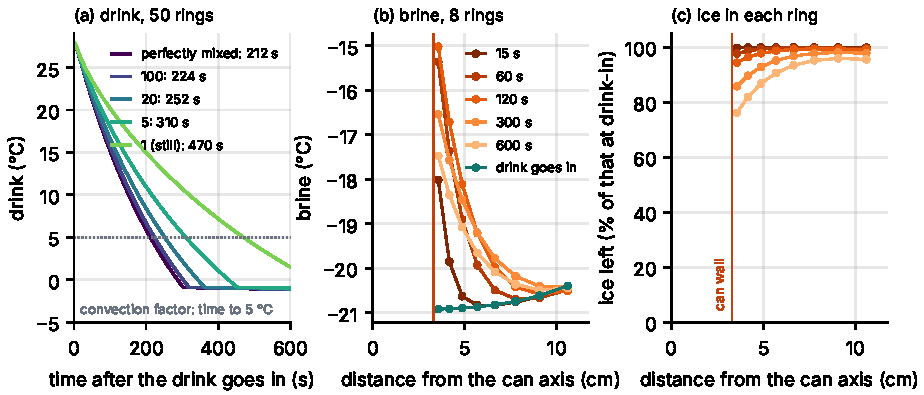
\includegraphics[width=\linewidth]{figs/f9_spreading.pdf}
\caption{Heat spreading through the bath. (a) The drink for convection factors from perfectly
mixed to still brine, run with 50 rings. (b) Brine temperature in each of the 8 rings, and
(c) the share of each ring's ice still there, at times after the drink goes in; the default
inputs. \code{python3 b8\_simple.py -{}-report-figure} redraws it.}
\label{fig:spread}
\end{figure}

With the defaults the drink reaches 5\,°C in \textbf{246\,s instead of 212\,s}. The inner ring
warms 5\,K above the rest within a minute and peaks at $-15.0\dC$, while the bulk barely moves
($-20.40$ to $-20.38\dC$); the ice next to the can goes first (Fig.~\ref{fig:spread}c: a quarter
of it in 10 minutes, against 4\,\% at the walls). Even before the drink, the bath is not uniform:
the glass warms the outer ring, so the brine there is 0.3\,K warmer than in a perfectly mixed bath.

\begin{center}\small
\begin{tabular}{@{}l c c c c@{}}
\toprule
$f$ & \multicolumn{2}{c}{time to 5\,°C} & brine by the can, peak & bath at drink-in \\
 & 8 rings & 50 rings & 8 rings & 8 rings \\ \midrule
$\infty$ (perfectly mixed) & 212\,s & 212\,s & $-19.7\dC$ & $-20.70\dC$ \\
100 (stirred) & 222\,s & 223.5\,s & $-18.3\dC$ & $-20.63\dC$ \\
\textbf{20 (default)} & \textbf{246\,s} & \textbf{252\,s} & $\mathbf{-15.0\dC}$ & $\mathbf{-20.40\dC}$ \\
5 & 286.5\,s & 310\,s & $-10.6\dC$ & $-19.94\dC$ \\
1 (still brine) & 364.5\,s & 470\,s & $-5.1\dC$ & $-19.34\dC$ \\
\bottomrule
\end{tabular}
\end{center}

\textbf{Rings.} The rings need to resolve $\ell$ \eqref{eq:pen}. At the default, 4, 8, 16, 32 and
50 rings give 239, 246, 249.5, 251 and 252\,s, so 8 are within 3\,\%. In still brine $\ell$ is
0.6\,cm and shrinks as the ice by the can melts away, so 8 rings (364.5\,s) are far from the 50-ring
470\,s; use 50 for $f$ below about 5.

\textbf{What it changes.} Over plausible ranges the inputs that move the time to 5\,°C most are
$h_o$ ($\div 3$ to $\times 3$: 497 to 160.5\,s), a measured $U$ (120–200\,W\,m$^{-2}$K$^{-1}$: 323 to 207.5\,s),
the drink's mass or heat capacity ($\pm 20$\,\%: 295.5 to 196\,s) and now $f$ (5–100: 286.5 to 222\,s);
then the headspace of §\ref{sec:level} (0.6–2.0\,cm: 236 to 260\,s).
The \FLOOR\ numbers hardly move. A fit of $U$ from a drink run (E3) now depends on where the
brine probe is: \textbf{within about 5\,mm of the can it measures the can alone}; out in the bath
it measures the can and the spreading together, and should be used with $f = \infty$. Two brine
probes, one at the can and one at least 5\,cm away, measure $f$: the default predicts a peak
difference of about 5\,K, still brine 14\,K, a stirred bath 2.4\,K.

\textbf{Still left out.} Each ring has one temperature from floor to surface, so the vertical
stratification of §9 is not in it. Convection is a fixed multiple of $k_b$, not a flow driven by
the temperatures it carries. And the rectangular tank is taken as a cylinder of the same floor
area.

\subsection{The box is not a perfect insulator}
\label{sec:box}
The room is 48\,K warmer than the bath, so heat leaks in through the styrofoam the whole time.
The model counts four paths from the room, each starting with the room's air film on the foam
($h = 9$\,W\,m$^{-2}$K$^{-1}$, convection and radiation):
\begin{center}\small
\begin{tabular}{@{}l r@{}}
\toprule
Path & Leak \\ \midrule
foam walls $\to$ air gap $\to$ tank glass $\to$ brine & 0.20\,W\,K$^{-1}$ \\
foam floor $\to$ tank glass $\to$ brine (the tank stands on the foam: no air gap) & 0.07\,W\,K$^{-1}$ \\
foam lid $\to$ still air $\to$ brine & 0.05\,W\,K$^{-1}$ \\
gaps $\to$ brine: lid seam, the lid's thin lip, holes for probe leads & 0.02\,W\,K$^{-1}$ \\ \midrule
all of them & 0.34\,W\,K$^{-1}$ \\
\bottomrule
\end{tabular}
\end{center}
The foam conducts 0.035\,W\,m$^{-1}$K$^{-1}$ through 30\,mm and holds 280\,J\,K$^{-1}$, so a box that starts
at room temperature gives up about 6\,kJ as it cools. The gaps are an estimate: buoyancy-driven
exchange through a 1\,mm seam round the lid carries about 0.01\,W\,K$^{-1}$, a 5\,mm one about 0.05.
The \code{b8\_sim.py} figure of 0.46\,W\,K$^{-1}$ (§8) left out the air films.

Next to the can's 4.3\,W\,K$^{-1}$ the leak is small: a box leaking anything from 0.25 to
1.0\,W\,K$^{-1}$ gives 246\,s to 5\,°C, within half a second. It shows in the bath instead: by the end
of the 50-minute run the default bath is at $-19.3\dC$ with 2.10\,kg of ice left, against $-17.6\dC$
and 1.94\,kg at 1.0\,W\,K$^{-1}$. A real box leaks more than the sum says (thin spots, seams, damp or
light foam), so it should be measured. \textbf{The box test}: 5\,kg of cold water from the fridge
in the tank, no ice or salt, the lid on with the probe leads through their usual gaps, logged for
3\,h and stirred before each reading. After the first 30\,min, while the room-temperature glass
warms the water, the water approaches the room exponentially:
\begin{equation}
(UA)_{\text{box}} = \frac{C}{t_2 - t_1}\,\ln\frac{T_{\text{room}} - T(t_1)}{T_{\text{room}} - T(t_2)},
\qquad C = m_w c_w + C_{\text{glass}} = m_w \times 4190 + 2020\ \text{J\,K}^{-1}.
\label{eq:boxtest}
\end{equation}
The model predicts 6.7\,°C at 30\,min and 9.4\,°C at 3\,h, and \eqref{eq:boxtest} applied to its own
curve gives back its leak to 1\,\%. \code{box\_test.toml} sets this run up in the simulator; a
measured value goes into \code{[box] measured\_UA}, which scales every path to add up to it.

\subsection{Inputs and the simulator}
Every number the simulator uses is in \code{inputs.toml}, with its unit and a tag saying where it
comes from (measured, to measure, assumed, literature, choice, model switch); a short file with
only the lines that change overrides it. \code{b8\_app.py} puts the main inputs on sliders with a
live drawing of the tank, the brine drawn ring by ring so the warm layer by the can shows. Every
slider has a box beside it: a number typed there and confirmed with Enter is used exactly, even
outside the slider's range, which then widens to follow it. The convection factor and the box's
measured leak have sliders of their own, and \code{inf} typed in the convection factor's box gives
the perfectly mixed bath. The web page
(\url{https://darkpyxlz.github.io/sypt/}) runs the same Python files unchanged in the browser
(Pyodide), with the same sliders and boxes, every input of \code{inputs.toml} editable, and
scenarios saved as \code{.toml} files or links. A run takes about 0.5\,s in Python and 1\,s in the
browser.

% ---------------------------------------------------------------- 13
\section{Literature}

Marked \secsrc where only a secondary or abstract-level source has been read.

Bodnar, R.\,J., \emph{Geochim. Cosmochim. Acta} \textbf{57}(3), 683–684 (1993) — the liquidus,
\eqref{eq:bodnar} \secsrc (equation via the Lille fluid-inclusion resource; original pages still to be
read). Swenne (1983), PhD thesis, TU Eindhoven — $T_E = 252.03$\,K, peritectic.
Drebushchak, Ogienko \& Yunoshev, \emph{Thermochim. Acta} \textbf{647}, 94–100 (2017) —
metastable eutectic near $-27\dC$, hydrohalite formation enthalpy. Chem.\ Eng.\ Educ.\
beverage-bottle study (WPI) — unstirred $h_o$, $h_i$, wall Biot numbers. SINTEF can data —
the $\tau$ behind $U_0$. Schulze Grachtrup, arXiv:1702.07014 (2017) — bottle benchmarks
for comparison. Koefod (2017) — mixing raises the dissolved share of salt, supporting §9 \secsrc.
Xu, Bootsma, Verzicco, Lohse \& Huisman, \emph{J. Fluid Mech.} \textbf{1019}, A11 (2025), and
Yang, Howland, Liu, Verzicco \& Lohse, \emph{J. Fluid Mech.} \textbf{969}, R2 (2023) —
mechanism only; both lie an order of magnitude below the bath's salinity. Sigma-Aldrich
solubility table — the source of the fit in \code{sypt code}. Purdue thermochemical table —
$\Delta h_s$ \secsrc.

\emph{For §\ref{sec:spread}.} Melinder, Å., \emph{Properties of Secondary Working Fluids for
Indirect Systems}, 2nd ed., IIR (2010) — $c_b$, $\rho_b$ and $k_b$ of NaCl brine, fitted from
its tabulation as implemented in CoolProp (INCOMP::MNA) \secsrc. IAPWS R10-06 (2009), Revised
Release on the Equation of State 2006 for H$_2$O Ice Ih — $c_i(T)$. Holland, D.\,M. \& Jenkins, A.,
\emph{J. Phys. Oceanogr.} \textbf{29}, 1787–1800 (1999) — the three-equation ice/brine interface
behind the \code{salt-limited} option \secsrc. Churchill, S.\,W. \& Chu, H.\,H.\,S.,
\emph{Int. J. Heat Mass Transfer} \textbf{18}, 1323–1329 (1975) — free convection on a vertical
wall, for $h_o$. Cheng, P. \& Minkowycz, W.\,J., \emph{J. Geophys. Res.} \textbf{82}, 2040–2044
(1977) — free convection from a vertical wall in a porous medium \secsrc. Carman, P.\,C.,
\emph{Trans. Inst. Chem. Eng.} \textbf{15}, 150–166 (1937) — the Kozeny–Carman permeability
\secsrc. Pyodide (\url{https://pyodide.org}) — Python in the browser, for the web simulator.

% ---------------------------------------------------------------- 14
\section{Notes for whoever picks this up}

\textbf{Do first.} E1. It costs one afternoon and decides between $-17.8$ and $-21.2\dC$ for
every later run, and whether the bath in E3 is a thermostat or a drifting reservoir.

\textbf{Do not} quote the rig-note charge as buffered; do not invert a blank run with $L_f$;
and do not report a single latent-heat share without the starting temperature of the water.

\textbf{The sharpest predictions}, cheapest first: the rig-note charge settles near $-17.8\dC$
with no crystals left; the original \code{sypt code} charge leaves only about 50\,g of ice;
the buffered bath holds $-21.2\dC$ for about 2.5\,h on the leak alone; a stalled one-shot bath
is colder at the floor than in the bulk.

\textbf{Software.} Python 3 with NumPy and SciPy; Matplotlib for the figures. Everything runs
in about 12\,s. The simulator (\code{b8\_model.py}) needs only Python 3.11 or later, plus
Matplotlib for its pictures; one run takes about 0.5\,s.

% ---------------------------------------------------------------- A
\appendix
\section{Using the code}

\begin{lstlisting}[numbers=none, frame=none, backgroundcolor=\color{teall}, language=bash]
python3 b8_sim.py           # checks, then figs/*.pdf and numbers.json
python3 b8_sim.py --quick   # checks only
python3 b8_simple.py        # the simulator (section 12), one run: table, summary, picture
python3 b8_app.py           # the simulator behind sliders, each with a box to type into
python3 b8_simple.py --report-figure   # redraws figs/f9_spreading.pdf
python3 test_b8.py          # the simulator's checks
\end{lstlisting}

\begin{lstlisting}[numbers=none, frame=none, backgroundcolor=\color{teall}]
import b8_sim as B
B.mix(1.0, 2.0, 0.5, T_water=25)         # adiabatic mix -> dict(T, m_ice, w, s_solid, regime)
B.mix_charge(B.BUFFERED)                 # a named rig charge
r = B.run_charge(B.UNBUFFERED, t_end=1500, drink=dict(law='power'))
B.time_to(r, 5.0)                        # seconds to 5 C
B.simulate(0.15, 0.06, 0.038, with_drink=False, k_diss=2e-3)   # kinetic dissolution
\end{lstlisting}

Constants marked \code{ASSUMED} in the source are the ones to replace with measurements: $c_i$,
$c_b(w)$, $\Delta h_s$, the hydrohalite solubility line, the drink's $c$ and can mass, and $U_0$.
To use a measured bath trace instead of the bath model, set \code{constant\_bath=True} and
replace the line that sets \code{T\_b} in \code{simulate()} with an interpolation of the log.

The heart of the model, \eqref{eq:H} and the solve of §4.3:
\lstinputlisting[firstline=111, lastline=189, firstnumber=111]{b8_sim.py}

\end{document}
